\subsection{Part B: Real-CV results}
\label{sec:results-b}

\subsubsection{Detection rate versus marker size and range}

Detection is governed by the apparent size in pixels, with a sharp floor. Across all four size groups, the rate is zero below 21~px, transitional in the 21 to 28~px bin (0.21 to 0.59 depending on size), and above 0.85 from 38~px upward (Figure~\ref{fig:det-px}). The $\sim$27~px 50\% budget measured independently in Section~\ref{sec:results-turbidity} crosses each group's curve near its 0.5 point. On the derived metric axis, the overall on-axis rates are 0.93 for the 149.4~mm markers, 0.61 at 74.7~mm, 0.43 at 44.4~mm and 0.29 at 35.6~mm over the swept range. The oblique run (median incidence of 58$^\circ$) detected only the 149.4~mm markers, at 0.60 overall, while the three smaller groups produced zero detections in 791 trials. Oblique viewing therefore costs roughly one size class, even before the angle reaches the detector's geometric limits.

\begin{figure}[H]
    \centering
    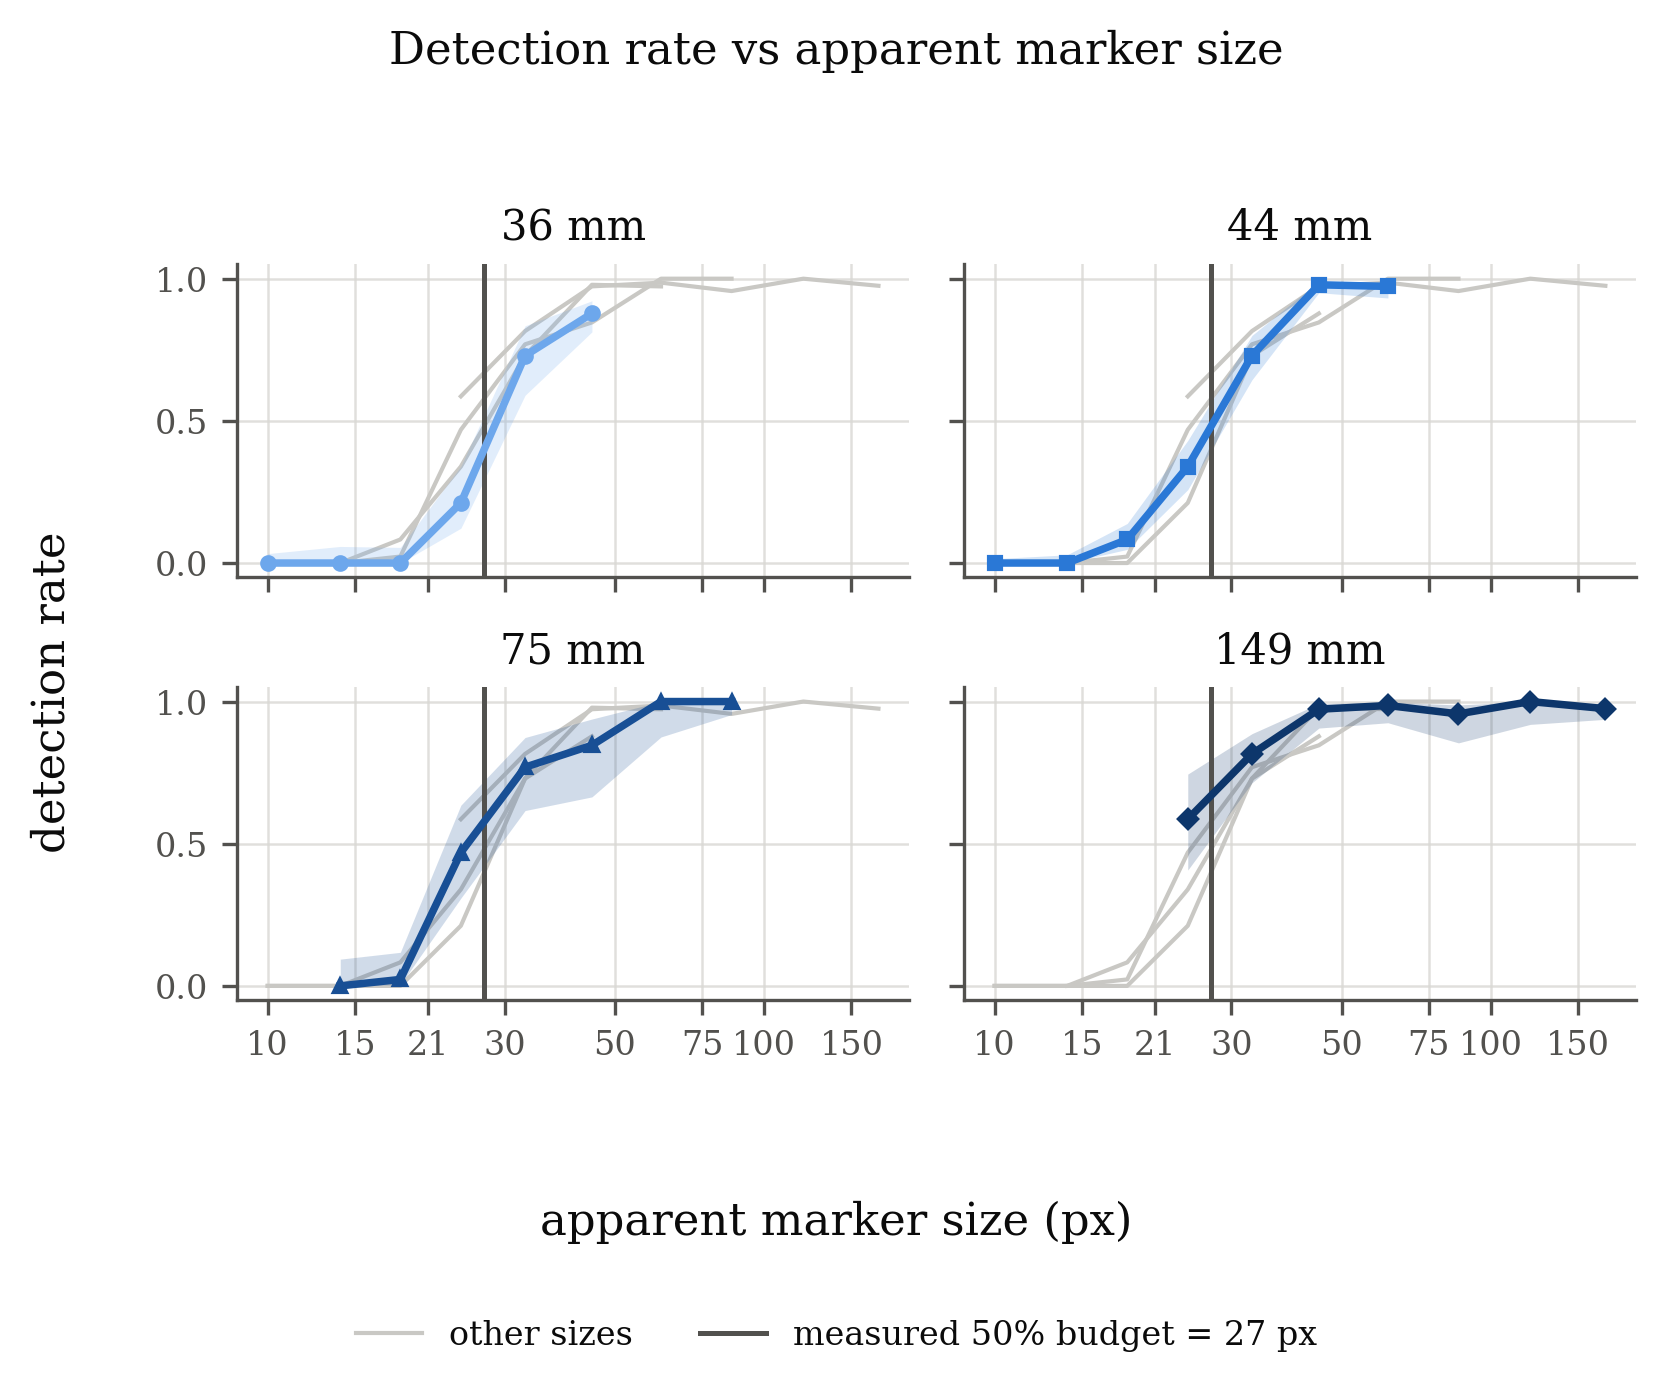
\includegraphics[width=0.95\textwidth]{Figures/detection_rate_vs_px.png}
    \caption{Detection rate versus apparent marker size per size group, with
        Wilson 95\% intervals, and bins with fewer than ten trials are suppressed.
        The vertical line is the $\sim$27~px 50\% budget
        (Section~\ref{sec:results-turbidity}).}
    \label{fig:det-px}
\end{figure}

\subsubsection{Maximum detection range}

The uncensored maximum detection ranges scale linearly with the marker side, measuring 5.10 and 4.87~m for the two 149.4~mm markers, 3.05~m at 74.7~mm, 1.55 to 2.17~m at 44.4~mm, and 1.10 to 1.14~m at 35.6~mm, fitted by $\mathrm{max\ range} \approx 34.9 \times \mathrm{side}$ (Figure~\ref{fig:max-range}). The walk-back continued approximately 3~m past the last detection with none recorded, so these are true detection limits. Two distinctions matter for a dock designer. First, only the largest markers reach the 5~m acquisition range assumed for the coarse phase, and only marginally. Second, the maximum range is a single-detection statistic, and the reliable (50\%) range sits lower. At 5~m, a 149.4~mm marker subtends 23.8~px, which is below the $\sim$27~px needed for 50\% detection (Section~\ref{sec:results-turbidity}). Its maximum range of 5.1~m therefore coexists with a 50\% range nearer 4.3~m, and it is the 50\% range that should size a dock. The measured law also validates the size assignment of the dock layout (Section~\ref{sec:method-layout}), since the largest markers alone carry long-range acquisition, while the interior small markers only need the close-range band they were placed for.

\begin{figure}[H]
    \centering
    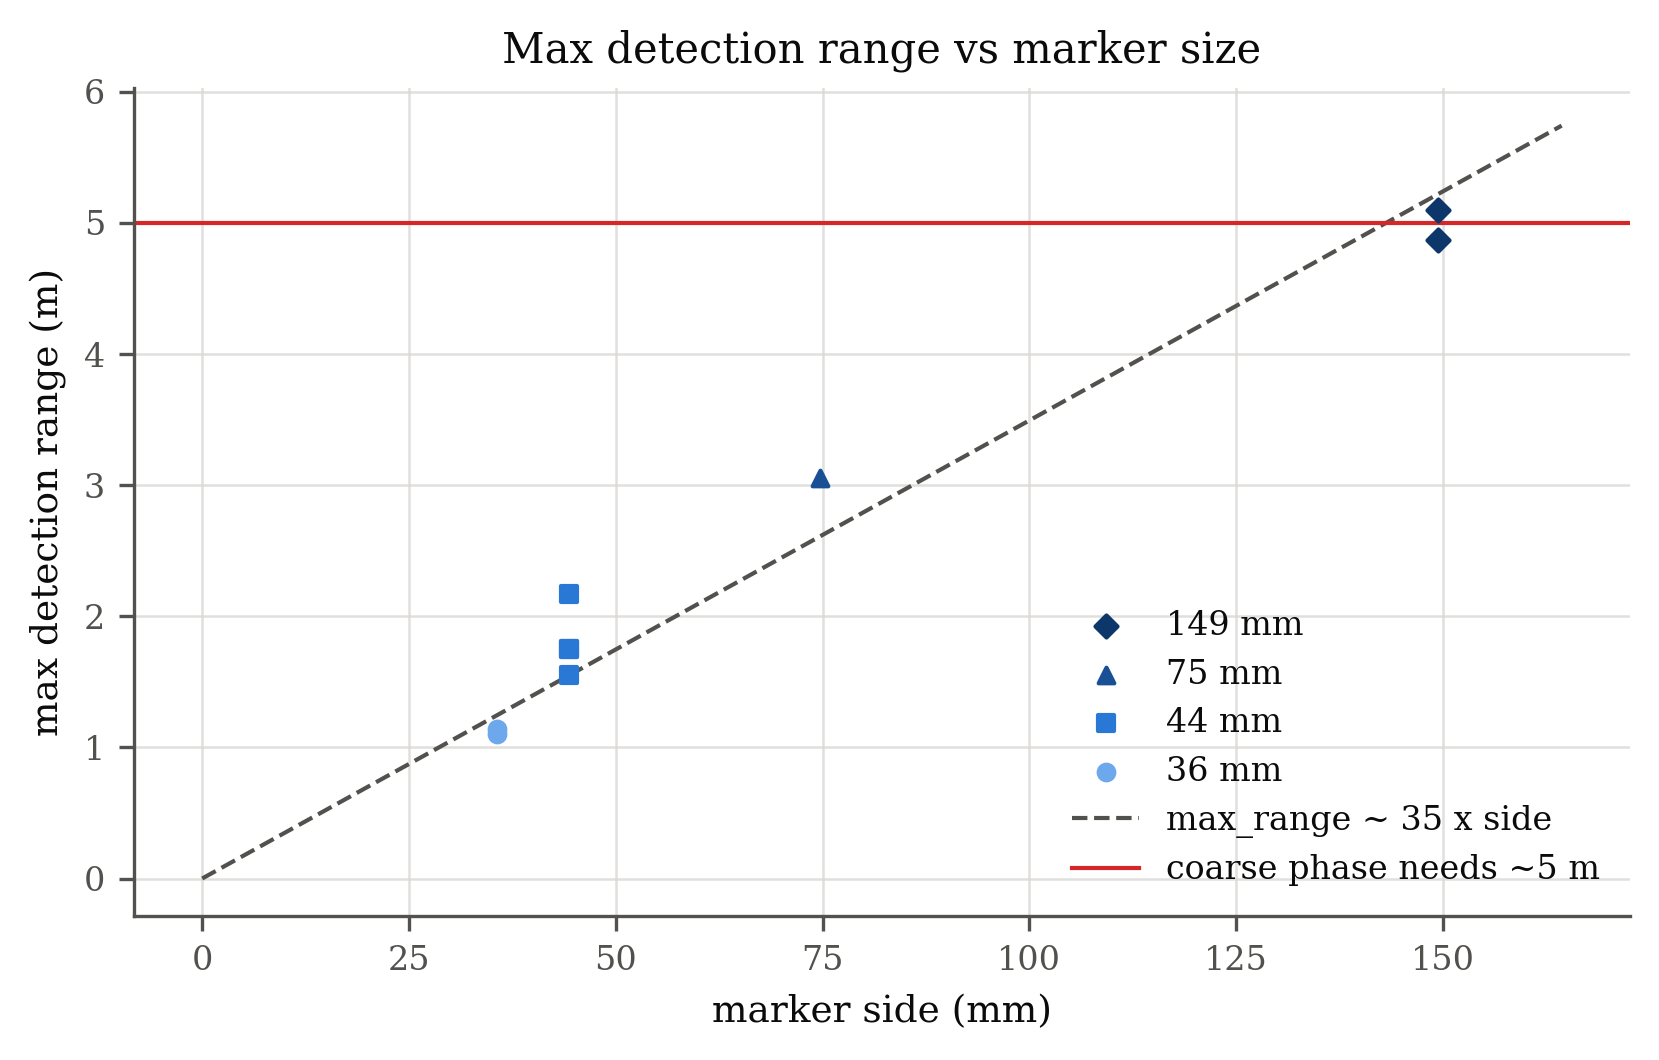
\includegraphics[width=0.8\textwidth]{Figures/max_range_vs_size.png}
    \caption{Maximum detection range versus marker side with the fitted
        linear law and the 5~m coarse-acquisition reference line.}
    \label{fig:max-range}
\end{figure}

\subsubsection{Pose self-consistency and misidentification}

With no external ground truth, the single-marker pose is scored against the leave-one-out board reference, which measures self-consistency instead of accuracy. The translation deviation grows from a 10.6~mm mean (9.4~mm jitter) in the 0.5 to 1.0~m bin to a 36.1~mm mean (32.9~mm jitter) at 2.0 to 3.0~m. The rotation deviation is 11 to 16$^\circ$ and roughly flat with range. These figures pool all marker sizes, since a per-size split would change the reference geometry with the marker under test. The sole camera-independent validation is the IMU gravity check, where over 323 frames, the board's estimated tilt from vertical has a median of 6.6$^\circ$, consistent with a hand-held, approximately vertical board. A yaw-rate cross-check was not corroborative (only 7 of the 25 turn segments had sufficient board coverage, and the vision magnitudes did not track the gyro), and it is reported as such. Misidentification was nearly absent in real water, with one off-board ID in 1376 on-axis detections (a rate of 0.0015) and none in the oblique run.

\subsubsection{Attenuation measurement}

The $B$-free contrast fit uses the instrument correction and per-marker intercepts over 934 samples spanning 0.62 to 3.19~m. It yields $\beta_b = 0.279$, $\beta_g = 0.247$, $\beta_r = 0.443$, $\beta_{grey} = 0.289$~m$^{-1}$ (with $r^2$ of 0.71, 0.67, 0.88 and 0.75, see Figure~\ref{fig:beta}). The strongest support for the correction chain comes from a quantity that was never used in the fit. The red-to-green attenuation ratio moves from 1.50 (raw) to 1.79 (corrected), against approximately 1.8 expected from water optics. A residual check over 5629 near-to-far marker pairs (not a statistical cross-validation, since no holdout was used) shows the exponential form predicts the real far-frame contrast to a median error of $-3.1$\% corrected, versus $+18.5$\% raw. At 5~m, this water gives a grey optical depth of $\tau = 1.44$, meaning 23.6\% of contrast survives. The fitted veiling light $B$ is not physically meaningful (negative $r^2$, and the green estimate exceeds the white sheet's own brightness). This is by design, since the method cancels $B$ from the contrast, and $B$ enters the synthesis only as a DC term that adaptive thresholding rejects.

\begin{figure}[H]
    \centering
    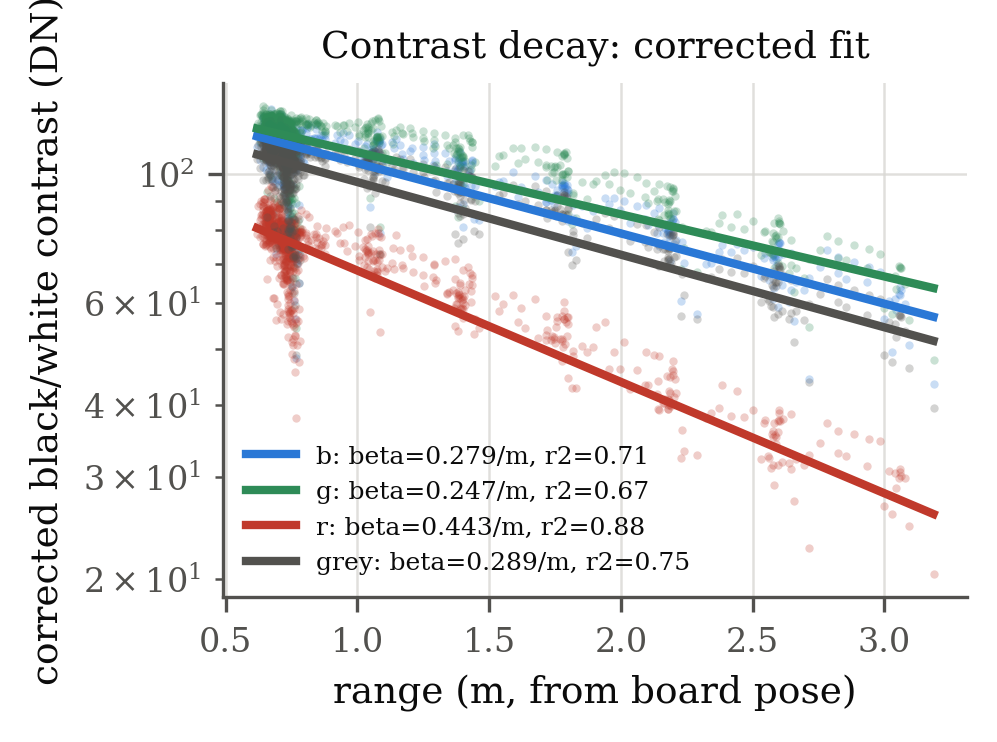
\includegraphics[width=0.8\textwidth]{Figures/beta_contrast_decay.png}
    \caption{Instrument-corrected black-to-white contrast versus range
        with the fixed-effects exponential fits per channel.}
    \label{fig:beta}
\end{figure}

\subsubsection{Turbidity envelope and marker sizing}
\label{sec:results-turbidity}

Re-attenuating all 2551 on-axis trials at the ten turbidity multipliers (a fixed denominator at every level) maps the detection envelope over apparent size and total optical depth (Figure~\ref{fig:surface}). The envelope has two regimes. Below $\tau \approx 2$, the boundary is vertical, meaning detection is pixel-limited and turbidity hardly moves it. Above $\tau \approx 2.3$, the boundary is horizontal, where detection collapses at every apparent size sampled, so it is turbidity-limited. The pixel budget quantifies the first regime. The apparent size needed for 50\% detection is 27.3 to 28.1~px, flat across a sevenfold span of optical depth ($\tau$ 0.18 to 1.30), and it only rises within the resolution of the binning before the collapse (Figure~\ref{fig:pxbudget}). ArUco's adaptive thresholding therefore keeps detection insensitive to contrast loss until an abrupt threshold near $\tau \approx 2$, where the failure is a cliff and not a gradual decline. Apparent size and turbidity are the same pair of governing variables identified by dos Santos Cesar et al.'s tank evaluation, which reported the smallest detectable size growing with turbidity at six discrete levels \cite{cesar2015evaluation}. The $\tau$-resolved envelope here refines that picture into a flat pixel-limited regime followed by an abrupt collapse.

\begin{figure}[H]
    \centering
    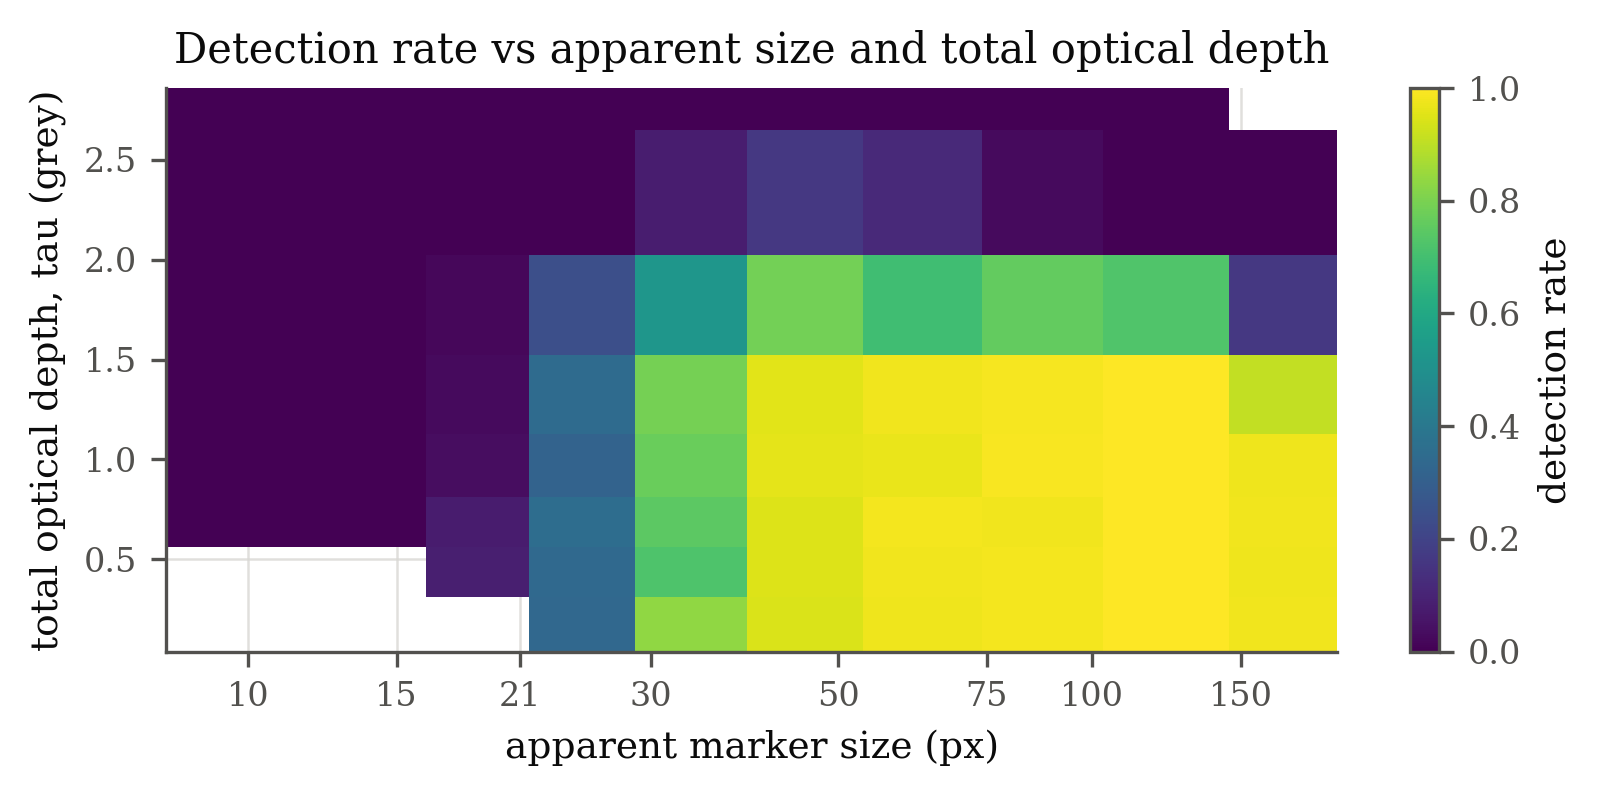
\includegraphics[width=0.9\textwidth]{Figures/rate_px_tau_surface.png}
    \caption{Detection rate over apparent size and total optical depth,
        where white cells are unreachable combinations.}
    \label{fig:surface}
\end{figure}

\begin{figure}[H]
    \centering
    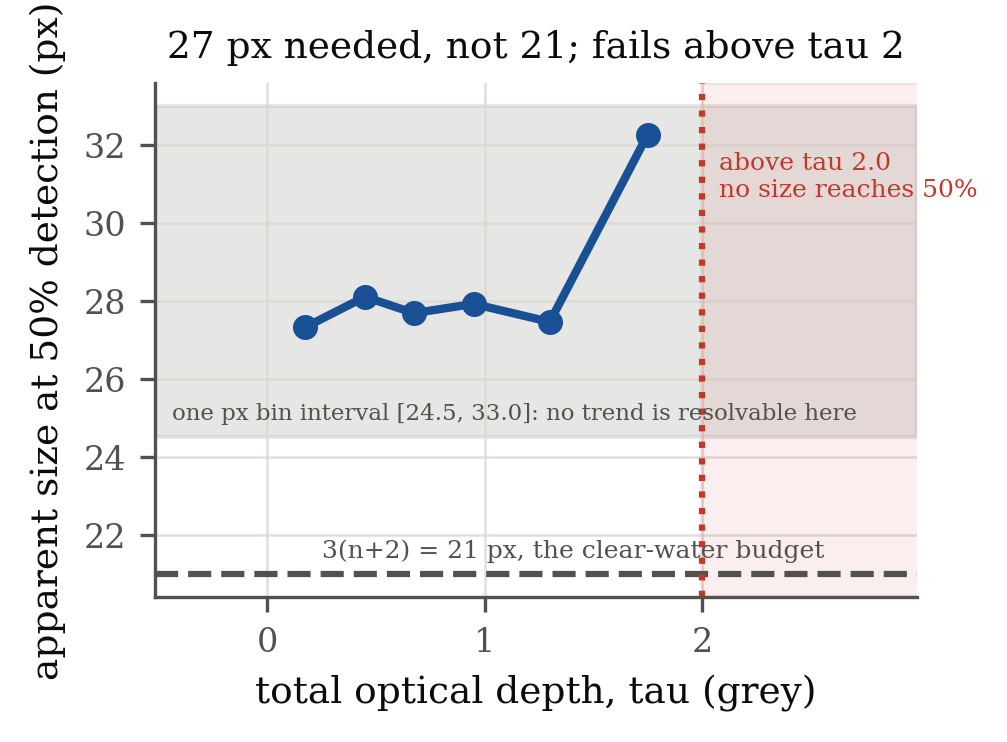
\includegraphics[width=0.6\textwidth]{Figures/px_required_vs_tau.png}
    \caption{Apparent size required for 50\% detection versus total optical
        depth, flat at $\sim$27~px up to $\tau = 1.3$. Above $\tau = 2$
        (dotted line, shaded region) no measured size reaches 50\%. The grey
        band is the single pixel-bin interval (24.5 to 33.0~px) within which
        the crossing is interpolated, so no trend narrower than the band is
        resolvable.}
    \label{fig:pxbudget}
\end{figure}

Inverting the pixel budget through the pinhole model sizes the dock marker. For 50\% single-frame detection, this pool's water requires a 105~mm marker at 3~m and a 182~mm marker (interval 154 to 207~mm) at 5~m. In clearer water ($\beta = 0.15$~m$^{-1}$), the 5~m requirement barely drops (174~mm), which confirms that below the cliff the requirement is set by pixels and not by the water. In murkier water ($\beta \geq 0.6$~m$^{-1}$, $\tau \geq 1.8$ at 3~m), the requirement is undefined within the measured envelope, since no marker size sampled achieves 50\%. The synthesised degradation is illustrated in Figure~\ref{fig:strip}. A forward-scatter check found no measurable edge blurring within apparent-size bins across the synthesised range (the slopes scatter around zero), so at these optical depths the operative mechanism is contrast loss and not blur.

\begin{figure}[H]
    \centering
    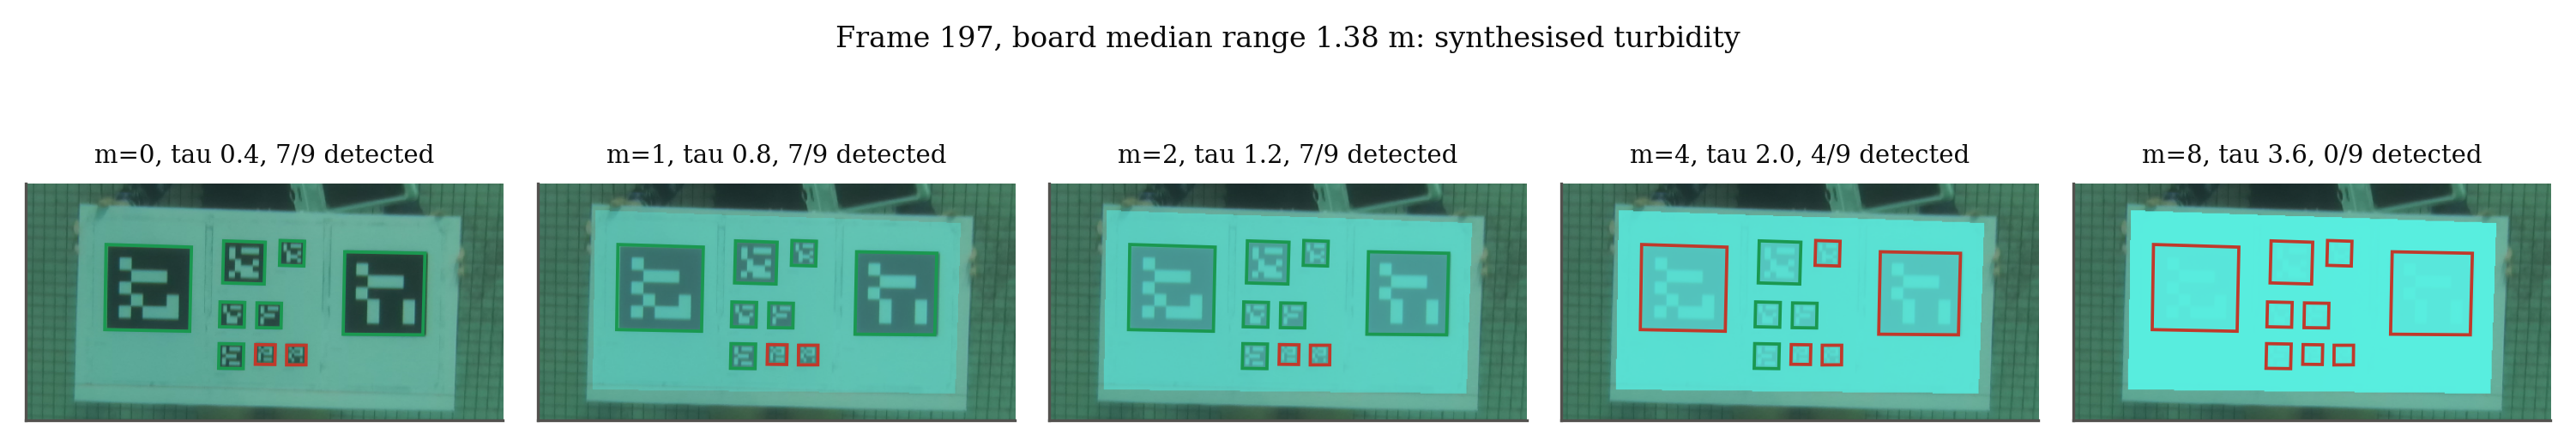
\includegraphics[width=0.95\textwidth]{Figures/synthesis_sweep_strip.png}
    \caption{One frame re-attenuated at increasing turbidity multipliers,
        detections outlined, with 7 of 9 markers at the real condition and 0 of 9 at
        the highest multiplier. The highest multipliers are diagnostic only, since
        their DC term is unphysical.}
    \label{fig:strip}
\end{figure}

\subsubsection{Preprocessing: CLAHE evaluated and rejected}

CLAHE was evaluated against the detector's own thresholding parameter over all 2551 trials at every turbidity level. In real water (multiplier 0), CLAHE is a net negative, with a detection rate of 0.512 versus the 0.519 baseline, while introducing 0.022 misidentifications per frame where the baseline has zero. Its apparent gain at high synthesised turbidity (0.337 versus 0.159 at the highest level) is measured on frames whose degradation adds no scattering noise, so it is an upper bound that remains unproven for real water. Lowering \texttt{adaptiveThreshConstant} to 3 recovers about two-thirds of that gap (0.276) at a third of CLAHE's misidentification rate (Figure~\ref{fig:preproc}). The engineering decision follows the real-water evidence, so there is no CLAHE stage in the pipeline and the detector's threshold constant is tuned instead.

\begin{figure}[H]
    \centering
    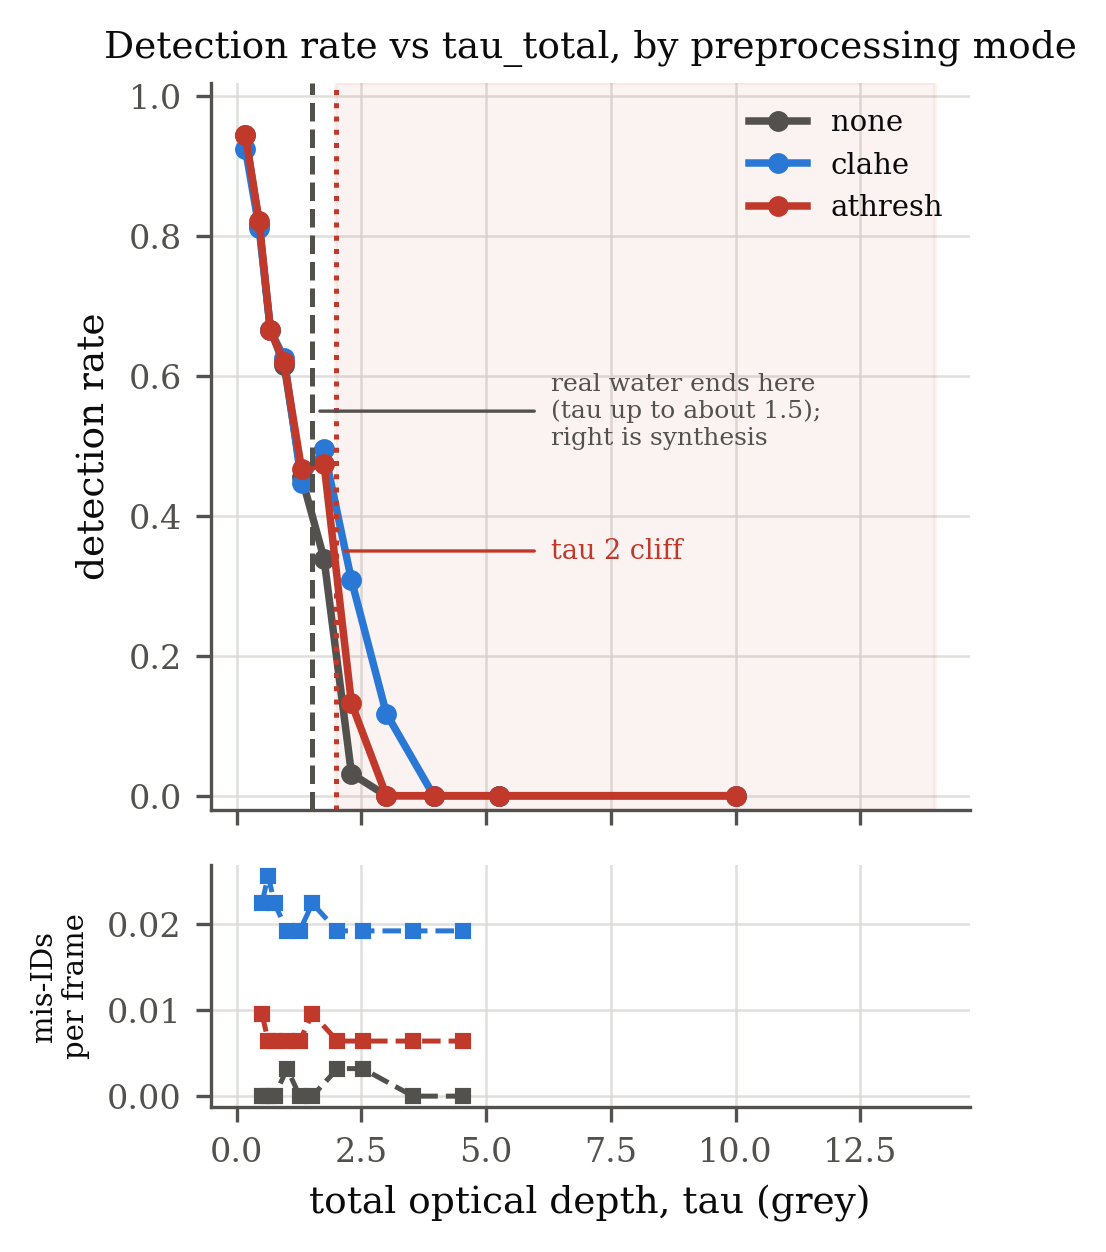
\includegraphics[width=0.6\textwidth]{Figures/preprocessing_eval.png}
    \caption{Detection rate (top) and misidentifications per frame
        (bottom) versus total optical depth for no preprocessing, CLAHE, and
        a lowered adaptive-threshold constant. Real water ends at the dashed
        line, and everything beyond is synthesised.}
    \label{fig:preproc}
\end{figure}

\subsubsection{Limitations}

The dataset is one pool and one session. The optical-depth axis is designed to generalise (results are reported against $\tau = \beta d$), but this water is a single point and the attenuation spectrum of other waters will differ. No external ground truth exists, so the pose results are self-consistency only, and all metric ranges carry $\pm$10\% from the in-air focal length. $\beta$ was fitted over 0.62 to 3.19~m, so quoting $\tau$ at 5~m assumes $\beta$ is constant with range. The oblique run is thin (161 detections, largest markers only) and the viewing angle was never controlled. The capture was hand-held, so motion blur is present and unmodelled. Finally, the synthesised turbidity levels derive from the same frames and are correlated samples, so the quoted confidence intervals understate the uncertainty at high multipliers.
